\section{Theoretical Background}
\label{sec:theoretical_background}
In this chapter, we introduce the theoretical background of the machine learning algorithms used throughout this thesis. We explain the different machine learning concepts and the purpose of \emph{classifiers}. Furthermore, we lay the foundations for the individual building blocks and layers of deep neural network systems. We explain the differences between \emph{convolutional neural networks} (CNN) and \emph{recurrent neural networks} (RNN) and continue by describing hybrid models composed of both of these. More specifically, we describe the \emph{convolutional recurrent neural network} (CRNN) architecture as used in this thesis. Finally, we present different representations of audio data suitable for machine learning tasks.

\subsection{Machine Learning}
Machine learning is a subfield of computer science that provides systems with the ability to automatically learn and improve from experience without being explicitly programmed. Machine learning relies on mathematical algorithms and statistics to find and learn patterns in data. 

\subsubsection{Types of Machine Learning}
The field of machine learning covers a multitude of different learning algorithms. While each of these is based on a different mathematical foundation, they also serve many different purposes. \emph{Classification} algorithms divide input data into two or more distinct classes. Each new input sample can then be assigned to one of these learned classes. For example, we could imagine an app that automatically classifies pictures of food and recognizes and names the respective dishes. While classification results are always discrete values, a \emph{regression} algorithm outputs continuous values instead. An example is a regressor predicting the future price of your favorite food based on historical price data. For other purposes, it is more important to know which data samples are similar to each other and form a group of their own. \emph{Clustering} algorithms divide data into groups and, unlike with classification, these group are usually not known before. For instance, a customer management system could cluster everyone into distinct clusters of different focus groups.

Regardless of an algorithm's purpose, machine learning typically can be divided into three categories from a high-level point of view:

	\begin{description}
		\item[Supervised Learning] is the task of building a machine learning model with labeled training data. Every data sample used during training is a pair consisting of a vector or matrix representation of the data and a label identifying the data as belonging to a certain class. Typically, a label is represented as a single number or a one-hot-encoded vector. Supervised learning algorithms learn an inference function mapping every data sample to its expected output label. A trained model should then be able to infer a suitable output class or value for new unknown data.

		\item[Unsupervised Learning] is the task of building a machine learning model with unlabeled training data. Unlike with supervised learning, none of the training samples include labels of the desired model outcome. Unsupervised learning algorithms learn a function by detecting the hidden structures inside the data. Many clustering algorithms fall into this category.

		\item[Reinforcement Learning] is the task of building a machine learning model without a set of classical training data. Instead, a reinforcement learning system is set within a specific environment and executes a set of actions. Each action's effect on the environment is measured, and reward is calculated. By maximizing this reward, the system finds actions that are most effective towards achieving the specified task. This setup is similar to computer simulations in other problem domains.
	\end{description}

The system described in this thesis is a supervised classification approach using a large-scale labeled training dataset.

\subsubsection{Classification}
\emph{Classification} in the context of machine learning refers to the task of assigning a data sample to the corresponding class. Classification algorithms are a form of supervised learning and, hence, need a training dataset of labeled data. The input to classifiers is referred to as \emph{features}. Classical machine learning algorithms, such as \emph{support vector machines} (\ac{svm}) and linear classifiers, usually require input features carefully designed by domain experts as a good representation of the original problem. This process is often referred to as \emph{feature engineering}. In contrast, deep learning classifiers such as \emph{neural networks} are able to directly work on the raw data representations. This has the benefit of building machine learning systems without the need for handcrafted features of domain experts but comes at the price of increased computational requirements. For computer vision tasks, for example, it used to be customary to train classical systems on preprocessed and extracted image features, such as SIFT key points~\cite{lowe1999object} or HOG descriptors~\cite{dalal2005histograms}. Deep learning systems, on the other hand, are capable of processing all the original raw pixels of the input image.


Figure \ref{fig:classifiers} shows an example of two binary classifiers dividing a simple dataset into two classes in 2D space.
%
	\begin{figure}[tp]
  		\centering
    	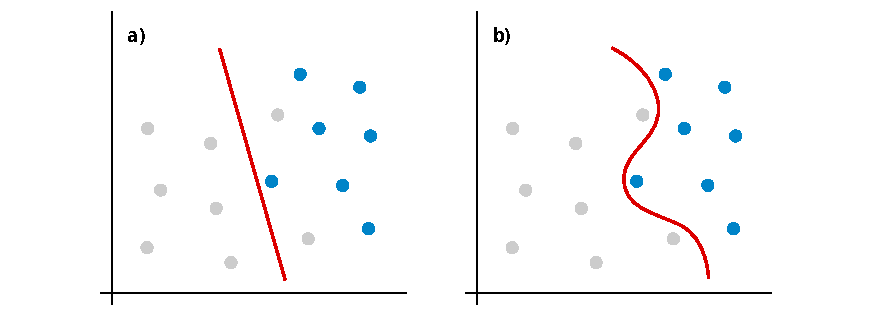
\includegraphics[width=\textwidth, keepaspectratio]{img/classifiers.pdf}
    	\caption{An example of two classifiers: A \emph{linear classifier}~(a) divides the data using a straight line but misclassifies two data points. A \emph{neural network}~(b) is able to learn a more complex decision boundary and separates the dataset without errors.}
    	\label{fig:classifiers}
	\end{figure}
%
On the left-hand side is linear classifier dividing all points along a straight line. While this sort of classifier is very easy to train and understand it lacks the necessary foundation to divide more complex datasets. On the right-hand side is a neural network (more details in the next section) featuring a more complex, yet more accurate decision boundary.

\subsection{Building Blocks of Deep Neural Networks}
Modern deep learning systems are composed in a layer-wise fashion. Each layer performs a nonlinear computation to extract features and learns a representation of the input data before passing on its outputs to the next layer in the architecture. The term \emph{deep learning} itself is not clearly defined but usually refers to having an at least two-layered model. Typical state-of-the-art systems have more than ten layers, some recent publications are even going as deep as \num{152}~layers~\cite{he2016deep}. While the total number of layers is, by no means, an indicator for an accurate and precise model, it makes capturing a larger and more generalized data representation possible.

\subsubsection{Neural Networks and Fully-Connected Layers}
While early \emph{neural networks} were inspired and named after discoveries in biology, particularly the neurons in animal brains, modern interpretations treat \emph{artificial neural networks} as a mathematical model of interconnected artificial neurons or a series of matrix operations~\cite{mcculloch1943logical, rosenblatt1958perceptron}.

\emph{Feedforward neural networks} are designed as a chain of layers, each applying an affine transformation. Each layer uses the output of the previous layer as an input, and all connections are directed without any self-references, $ f(\vecsym{x}) = f_i(f_{i-1}(...(f_1(\vecsym{x})))) $, where $\vecsym{x} \in \mathbb{R}^n $ is an input vector. The first and last layer are referred to as the \emph{input} and \emph{output} layer, respectively.

When fed with an input vector $x$, a neural network computes an affine transformation:
$$
f(\vecsym{x}, \matsym{W}, \vecsym{b}) = \sigma(\matsym{W}^T\vecsym{x} + \vecsym{b})
$$
where $\sigma$ is function $\sigma: \mathbb{R}^n \rightarrow \mathbb{R}^n$, $\matsym{W} \in\mathbb{R}^{n \times m} $ an $n \times m$ \emph{weight matrix}, and $\vecsym{b} \in\mathbb{R}^m $ a \emph{bias term}~\cite[p.~192]{Goodfellow-et-al-2016}. Both the weights and biases are trainable parameters and updated during the learning process. By itself, the chain of linear transformations can only model linear relations. To model more complex scenarios, $\sigma$ is a nonlinear \emph{activation function}. Typical candidates for activation functions in neural networks are \emph{rectified linear units} (\ac{relu})~\cite{nair2010rectified}:
$$
\sigma(\vecsym{x}) = \operatorname{max}(\vecsym{x}, 0)
$$

Within the deep learning community, neural networks are also referred to as \emph{fully-connected} layers (\ac{fc}), owing to the fact that each artificial neuron is connected to all outputs of the previous layer. Figure~\ref{fig:nn} shows an example of a three-layer neural network.
%
	\begin{figure}[tp]
  		\centering
    	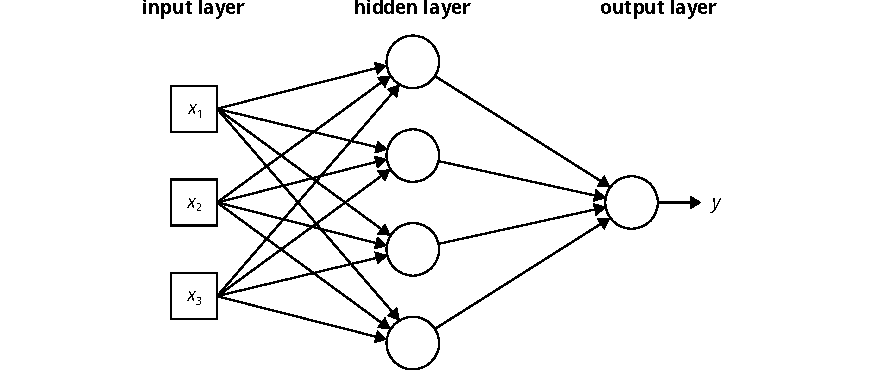
\includegraphics{img/nn.pdf}
    	\caption{A neural network with three layers. Each layer is connected to all outputs of the previous layer. All central layers, which are neither connected to the network's inputs or output, are referred to as \emph{hidden layers}. Note that all connections between the neurons are directed and do not include self-references. Therefore, we refer to these classes of models as \emph{feedforward neural networks}.}
    	\label{fig:nn}
	\end{figure}
%
Any layer not directly connected to the input or output is referred to as a \emph{hidden layer}. In our example, we only have a single output neuron and, hence, a binary classifier for the two classes. For multi-class tasks, we can add more output neurons. Typically, fully-connected layers are used as final layers of a deep neural network architecture serving as a classifier.

\subsubsection{Convolutional Layers}
\emph{Convolutional neural networks} (CNN) are simply neural networks that use convolution in place of general matrix multiplication in at least one of their layers. CNN specialize in processing data that has grid-like structure, such as the 2D grid of pixels of an input image as in our case. As the name suggests, they make use of the mathematical \emph{convolution} operation. For computer vision tasks this can be thought of as the weighted sum of all pixels in a neighborhood. More formally, convolution layers are expressed as \cite{sun2014deep}: 
%
$$
\matsym{Y}^{j(r)} = \sigma \left( \vecsym{b}^{j(r)} + \sum_i \matsym{K}^{ij(r)} \ast \matsym{X}^{i(r)} \right)
$$
%
where $\matsym{X}^i$ and $\matsym{Y}^j$ are the $i$-th input and $j$-th output map, respectively. $\matsym{K}^{ij}$ defines the kernel between those two maps and $\ast$ denotes the convolutional operation. $\sigma$ is an activation function, such as ReLU. $\vecsym{b}^j$ is the bias of the $j$-th output map and $r$ indicates a local region where weights are shared.

Typical kernels for CNNs have a square size of $3 \times 3$. Thus, for each pixel in the output map a neighborhood of $3 \times 3 = 9$ pixels is evaluated by the convolutional operation.  Figure~\ref{fig:convolution} shows the convolution of a single pixel in the output map $\matsym{Y}^{j}$.
	\begin{figure}[tp]
  		\centering
    	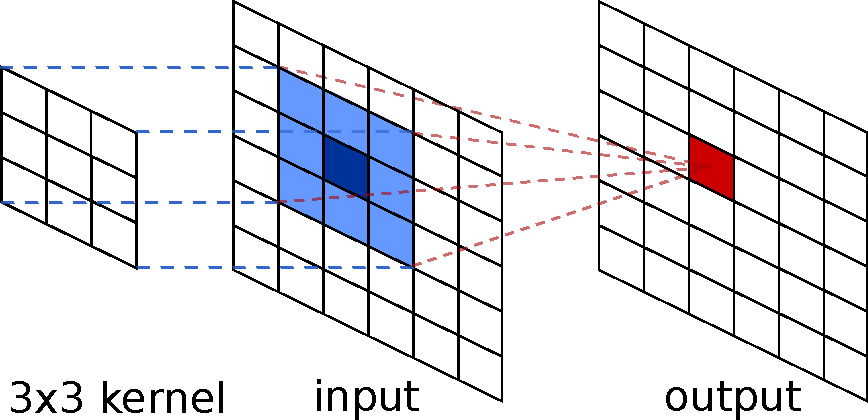
\includegraphics{img/convolution.pdf}
    	\caption{A convolution operation on an image using a $3 \times 3$ kernel. Each pixel in the output image is the weighted sum of \num{9}~pixels in the input image. The weights are not fixed but instead learned by the model.}
    	\label{fig:convolution}
	\end{figure}
	All pixels involved in the calculation of this pixel are referred to as its \emph{receptive field}. 

Kernels are learned during the training and can be thought of feature detectors. This concept is often used in the field of image processing where predefined kernels such as a Sobel filters are used for edge detection and Gaussian filters for blurring. Similarly, a CNN learns to detect simple features such as edges in lower layers. Convolutional layers at the end of the network architecture combine these simple  features to compound shaped features able to reliably identify an input. 

Typically, a CNN does not only learn one kernel but several, one for each desired output dimension. Other hyperparameters include the \emph{stride} and amount of \emph{zero padding}. The former defines by how many pixels the kernel is translated on the input. The latter specifies how to handle convolutions along the edge of an input where the kernel would need to include pixels from outside the image. Similarly to fully-connected layers, an nonlinear activation function is applied on the output of a convolutional layer as well.  

Unlike fully-connected artificial neural networks, CNNs need fewer parameters through the use of \emph{weight sharing}. A fully-connected neural network of $m$ inputs and $n$ outputs requires $m \times n$ weight parameters. A convolutional layer, on the other hand, each member of the kernel is used on every position of the input. Instead of learning parameters for every position in the input is only uses one set of $k \times k \times c \times o$ weights, where $k$ is the kernel size, $c$ the number of channels in the input, and $o$ the number of desired output channels (often called feature maps). For instance, a $100 \times 100 \times 3$ RGB color input image would require $100 \times 100 \times 3 \times 128 = 3840000$ weight parameters for a fully-connected layer with \num{128} outputs. In contrast, a CNN only uses $3 \times 3 \times 3 \times 128 = 3456$ weight parameters for a two-dimensional kernel of size $3 \times 3$ and for the same number of output units.


\subsubsection{Pooling Layers}
A convolutional layer is typically followed by a \emph{pooling} layer (sometimes also called subsampling or downsampling layer). Pooling layers are used reduced the spatial dimensions (width and height) on the input data. \emph{Max pooling}, for instance, only outputs the maximum value within its neighborhood. Similar to convolutions, pooling uses a $n \times $ kernel parameter to determine which input pixels are effected by the subsampling.

	While pooling leads to a reduction in information, this has two main benefits. First, pooling improves the computing efficiency of a network since next layers in the network architecture need to process less data. Typically, $2 \times 2$ pooling with a stride of \num{2} is used, effectively halving every input along the width and height dimension. 	
	Second, pooling helps against overfitting.
	
	Figure~\ref{fig:convnet} shows an example of a typical convolutional neural network constructed from convolutional, pooling and fully-connected layers.
		\begin{figure}[tp]
  		\centering
    	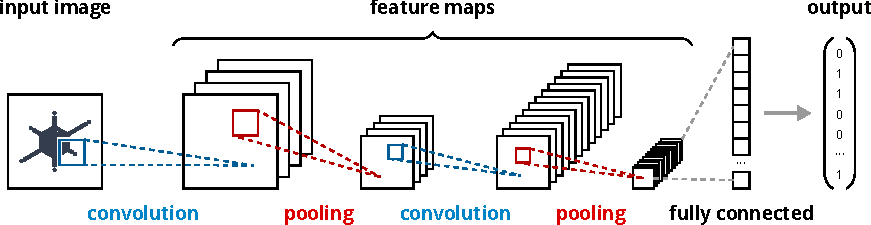
\includegraphics{img/convnet.pdf}
    	\caption{A typical \emph{convolutional neural network} architecture. An input image is fed through a series of convolutional and pooling layers. Each convolution extracts higher-level features and increases the number of feature maps. Each pooling layer subsamples the data, typically reducing the $x$ and $y$ dimension by half. A final, fully-connected layer serves as a classifier to predict the output value.}
    	\label{fig:convnet}
	\end{figure}
	Typically, an alternating sequence of convolutional layers followed by pooling layers is finalized by a fully-connected layer serving as a  classifier.

\subsubsection{Softmax Cross-Entropy Loss Function}
The \emph{softmax} function is an activation function applied to last layer to obtain probability distribution. It maps any $K \in\mathbb{N}^+$-dimensional input vector $\vecsym{x} \in\mathbb{R}^K$ onto a vector with a $[0, 1]$ value distribution, where the sum of all entries is \num{1}:
%
$$
\operatorname{softmax(}x\operatorname{)}_i= \frac{\exp^{x_i}}{\sum_{k=0}^K \exp^{x_k}}
$$
%
In order to train a neural network we constantly calculate the difference between a desired output class $y$ and a predicted class $\hat{y}$. We refer to such an error measure between the approximated and expected output value as \emph{loss function}. A commonly applied loss function for multi-class classification problem, as presented in this thesis, is cross-entropy loss:
%
$$
L_{cross\_entropy} = -log \left( \frac{\exp^{f_y}}{\sum_k \exp^{f_k}} \right)
$$
%
where $f_y$ is the probability granted to the correct class and $f_k$ are probabilities of all classes. Since part of the formula contains a softmax calculation we refer to this loss function as \emph{softmax cross-entropy loss}.

\subsubsection{Back Propagation Through Time}

\subsection{Recurrent Neural Networks}
\subsubsection{Long Short Term Memory Networks}

\subsection{Convolutional Recurrent Neural Networks}
\label{sec:hybrid_networks}
While both CNNs and RNNs can be used completely on their own, for some task it is worthwhile to use a combination of both. These \emph{hybrid networks} can combine the best of both worlds. Specifically, in this thesis we are using \emph{convolutional recurrent neural network} consisting of a CNN part and an RNN part. Tang et al. first introduced this architecture in the context of document classification \cite{tang2015document}.

The convolutional part is responsible for detecting and extracting local visual features into an intermediary audio representation. A recurrent part is tasked with temporal summarization of these features taking the global structure into account. Figure~\ref{fig:crnn} show the architecture of a CRNN network. 
%
	\begin{figure}[]
  		\centering
    	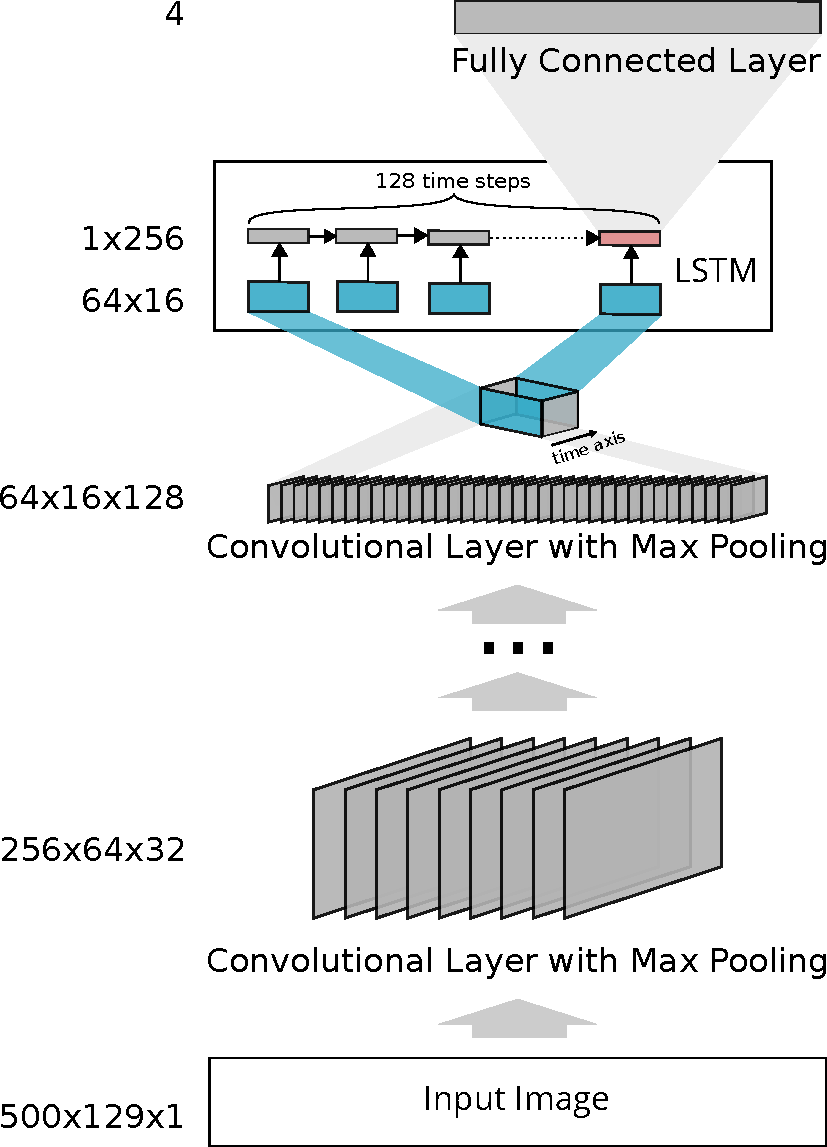
\includegraphics[]{img/crnn.pdf}
    	\caption{Our proposed CRNN hybrid network architecture consists of two parts. A CNN extracts local visual feature from our input images and outputs a intermediary representation of our audio frequencies. The output of the final convolutional layer is sliced along the time axis into time steps of frequency features for the LSTM. The output of the final LSTM time step is fed into a fully-connected layer for classification.}
    	\label{fig:crnn}
	\end{figure}
	%
	The last convolutional layer of a CNN is replace with a LSTM layer. In the context of language identification, the outputs of the last convolutional layer result in a tensor $t \times f \times c$, where $t$ are time steps, $f$ the frequency features, and $c$ the feature map outputs of the CNN. This tensor is stacked along the frequency dimension and split along the time axis into $t$ time step inputs of $ f \times c$ for the LSTM.
	
	For this thesis we use a bidirectional LSTM that performs both forward and backward pass a long the time sequence. We combine that last output of the forward pass with the first output of backward into a single, concatenated output. Finally, this is fed into a fully-connected layer serving as a classifier.
	
\subsection{Audio Representations}
There are many different representations for audio data. Many people are familiar with waveform representation which is usually represented as a plot of signal amplitude along a time axis. A raw waveform representation is typically not directly used as input to machine learning systems.
Other representations such as \emph{spectrogram} images or \emph{mel-frequency cepstral coefficients} (MFCCs) vectors are more common. To obtain both of these we need to transform the original audio signal.

First, we discretize the audio signal into into a list \emph{spectral vectors} (a spectrum) by applying a Fourier transformation. Each spectral vector consists of amplitude and frequencies pairs at a point in time. When visualizing these we get a spectrogram image as shown in Figure~\ref{fig:waveform}. 
%
	\begin{figure}[tp]
  		\centering
    	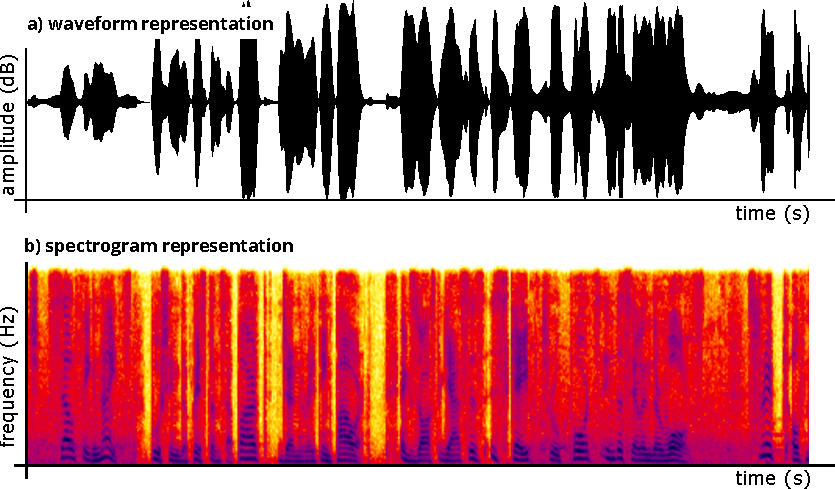
\includegraphics{img/waveform.pdf}
    	\caption{Different visual representations for a ten second audio file. a) shows a familiar waveform representation. b) shows the spectrum of frequencies known as spectrogram. Spectrogram images  are a commonly used representation for audio learning tasks.}
    	\label{fig:waveform}
	\end{figure}
%

The time domain is along $x$ axis and the frequency domain in Hz is along the $y$ axis. Additionally, the color intensity for each data point represents the amplitude or loudness value for a given frequency at that point of time. Spectrograms are especially useful for studying time--frequency features such as \emph{phonemes}. A phoneme is the smallest unit of sound expressing part of an word or single letters. While phonemes themselves are universally shared across different languages, their arrangement as a sequence forms the individual sounds and words distinctive to one language. Frequencies form phonemes which in turn form words. These can be combined to sentences or assemble the vocabulary of a language.
Within a spectrogram image we can clearly see distinct, bright, ripple-like patters, each representing a heightened frequency activation at that time. Due to the anatomy of the human vocal cords we emit sounds vibrating on multiple frequencies while speaking. 
The frequency axis is divide into multiple \emph{formants}, defined as a range of frequencies of a complex sound in which there is an absolute or relative maximum in the sound spectrum. There are several formants ranging form the lower speech frequencies to the higher ones. Voxels can be identified by their difference in the lower F1 and higher F2 format. Already, we note that there is a lot more information encoded into theses images then first meets the eye and, hence, a lot of speech processing systems use spectrograms.

MFCC is obtained by using linear cosine transform of log power spectrum on a nonlinear mel-frequency scale. This means that, first the powers of the spectrum are mapped onto the \emph{mel-scale}. The mel-scale groups frequencies onto a perceptual scale of equally distanced audio pitch values \cite{stevens1937scale}: 
$$
\vecsym{m} = 2595 \log_{10}\left(1+{\frac {f}{700}}\right)
$$
where $\vecsym{m}$ are the resulting mels and $f$ frequencies in Hz. The mel-scale is modeled after human ear's deficiency to differentiate adjacent frequencies. Effectively this groups frequencies together into bins with many, smaller bins for lower frequencies and only a few larger for the higher frequencies. Further, we calculate the powers of the mel-spectrum and apply the logarithm to these. The resulting energies are fed into a \emph{discrete cosine transformation} of which we keep the first 13 coefficients as our MFFC vector \cite{sahidullah2012design}. 
